\chapter{Экспериментальный раздел}
\label{cha:research}
    В данном разделе будут проведены эксперименты 
    для сравнительного анализа трёх алгоритмов по затрачиваемому процессорному 
    времени в зависимости от индекса слова в словаре.
    Тестирование проводилось на сервере
    под управлением Ubuntu Linux (64-bit) с 1 Гб оперативной памяти.

    \section{Сравнительный анализ на основе замеров времени работы алгоритмов}
        В рамках данного проекта были проведёны эксперименты
        по замеру времени работы алгоритмов поиска слова в словаре:
        \begin{enumerate}
            \item полным перебором (график \ref{graph:test:brute-force});
            \item двоичным поиском (график \ref{graph:test:binary});
            \item поиском по сегментам (график \ref{graph:test:segment}).
        \end{enumerate}

        В качестве словаря используется толковый словарь В. Даля Изд. "Цитадель", г. Москва, 1998 г.
        Всего в нём 2264828 слов, из которых 368274 являются уникальными. 
        Тестирование проводилось на уникальных словах с добавлением несуществующего.

        \begin{figure}[h!]
            \centering
                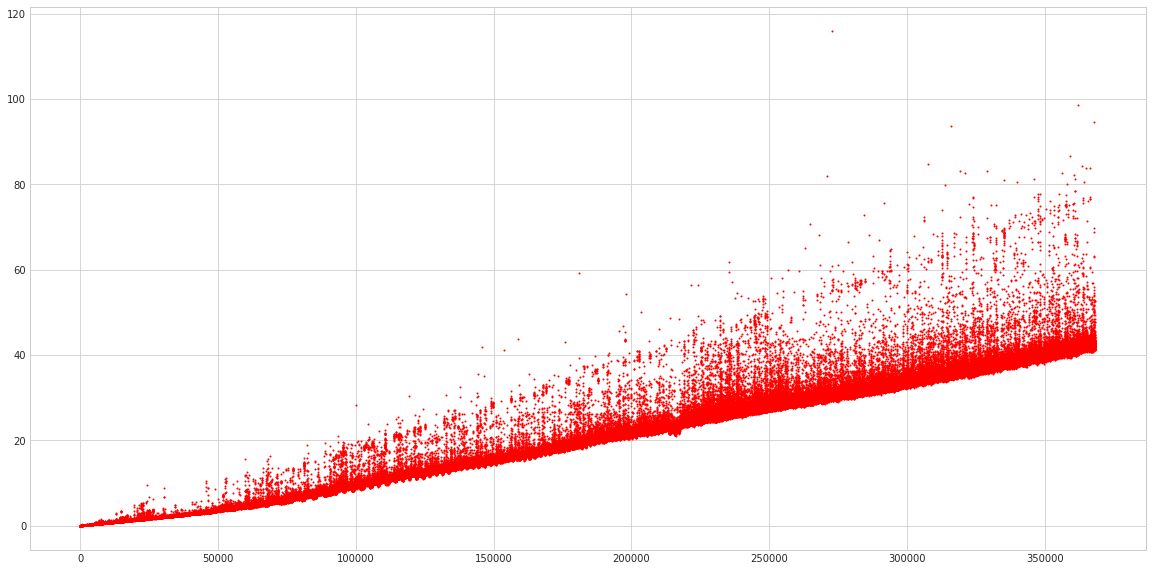
\includegraphics[angle=90, height=0.95\textheight]{BruteForce.png}
                \caption{Время поиска слова в словаре полным перебором}
                \label{graph:test:brute-force}
        \end{figure}


        
        \begin{figure}[h!]
            \centering
                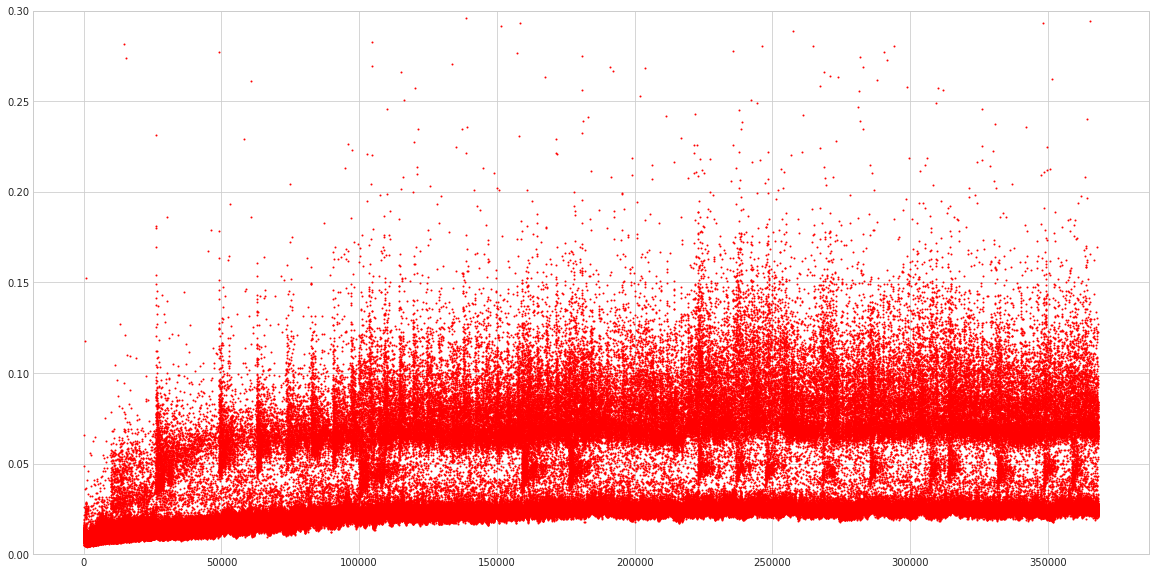
\includegraphics[angle=90, height=0.95\textheight]{BinarySearch.png}
                \caption{Время двоичного поиска слова в словаре}
                \label{graph:test:binary}
        \end{figure}

        \begin{figure}[h!]
            \centering
                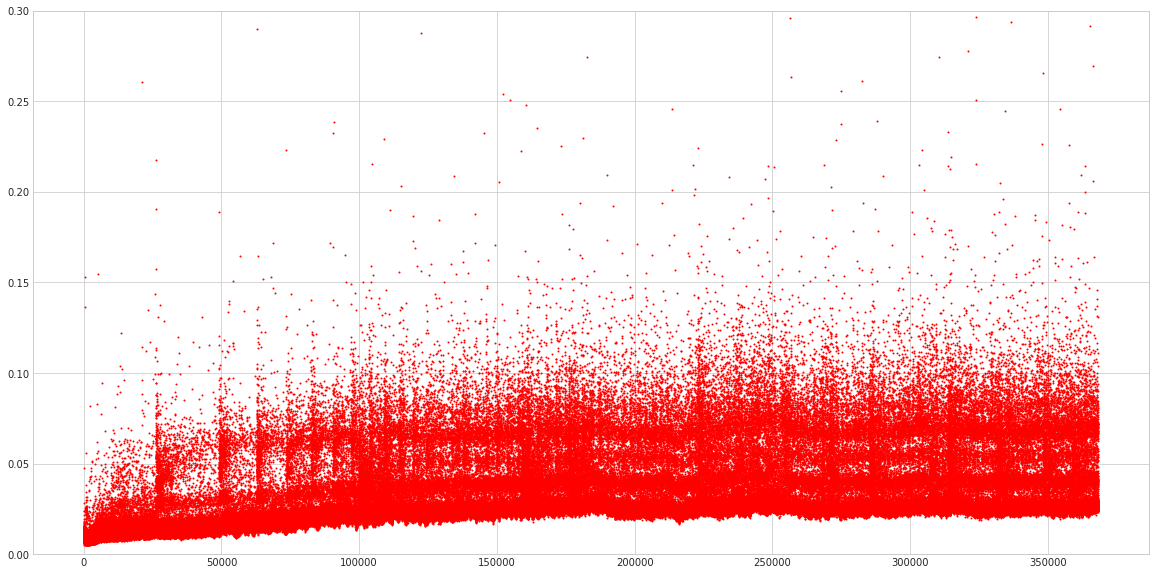
\includegraphics[angle=90, height=0.95\textheight]{SegmentSearch.png}
                \caption{Время поиска слова по сегментам в словаре}
                \label{graph:test:segment}
        \end{figure}

    \section{Статистический анализ замеров}
        По графику \ref{graph:test:brute-force} видно, 
        что преимущественно время поиска линейно, 
        но возможны случайные увеличения времени поиска 
        в связи с выполнением сервером других процессов.
        В худших случаях алгоритму требуется 42 секунды 
        на поиск последего из 368274 слов или же несуществующего. 

        На рисунке \ref{graph:analysis:frequency} приведён график
        плотности распределения времени поиска слова в словаре.
        В среднем бинарному поиску требуется 0.03577 секунд со 
        среднеквадратичным отклонением в 0.02748 секунд.
        В то время как алгоритму поиска по сегментам
        необходимо 0.03097 со среднеквадратичным отклонением в 0.0194 секунд. 
        Такой малый разброс значенией вызван распределением слов по первым буквам
        в словаре по сегментам (график \ref{graph:analysis:frequency:segment}). 
        Из-за этого время поиска остаётся примерно одинаковым.

        \begin{figure}[h!]
            \centering
                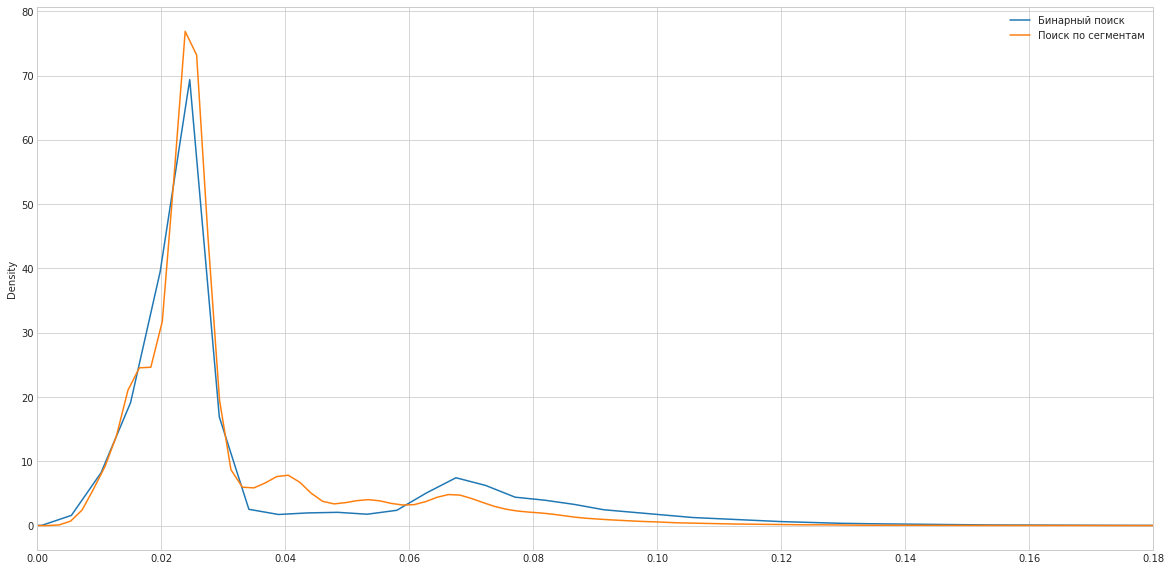
\includegraphics[angle=90, height=0.95\textheight]{frequency-analysis.png}
                \caption{Плотности распределения времени поиска слова в словаре}
                \label{graph:analysis:frequency}
        \end{figure}

        \begin{figure}[h!]
            \centering
                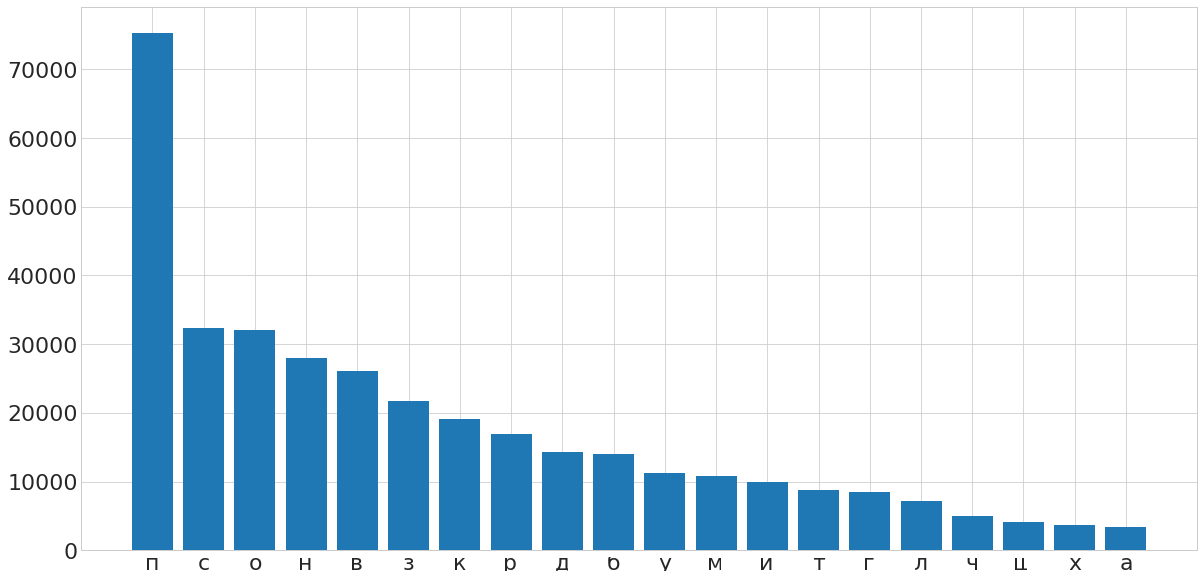
\includegraphics[angle=90, height=0.95\textheight]{SegmentFr.png}
                \caption{Распределение первых 20ти букв слов в словаре по сегментам}
                \label{graph:analysis:frequency:segment}
        \end{figure}

    \section{Вывод}
        В ходе экспериментов по замеру времени работы было установлено, что 
        самым эффективным и стабильным является поиск по сегментам.
        Самым долгим является алгоритм полного перебора.
        Его время возрастает каждый раз из-за того, 
        что слова находятся дальше в словаре, 
        а каждый раз поиск начинается с самого начала. 
        По графикам алгоритма бинарного поиска и поиска по сегментам 
        можно увидеть нормальное распределение времени поиска слова в словаре.
        На данных тестовых данных 

\newpage